On modélise l'altitude d'un projectile en fonction du temps $t$ exprimé en secondes par la fonction $f$ définie sur l'intervalle $[0~;~+\infty[$ par :
\[ f(t) = (2-0,5t)(7t+1) \]
où $f(t)$ est la hauteur, exprimée en mètres.

\begin{enumerate}
	\item
	\begin{enumerate}
		\item Vérifier que $f(t) = -3,5t^2 + 13,5t + 2$, pour tout $t$ appartenant à l'intervalle $[0 ; +\infty[$.
		\item Calculer $f(0)$ et interpréter $f(0)$ dans le contexte de l'énoncé.
	\end{enumerate}

	\item Ci-dessous, on donne une représentation graphique partielle de la fonction $f$ et son tableau de variation.

	\begin{center}
		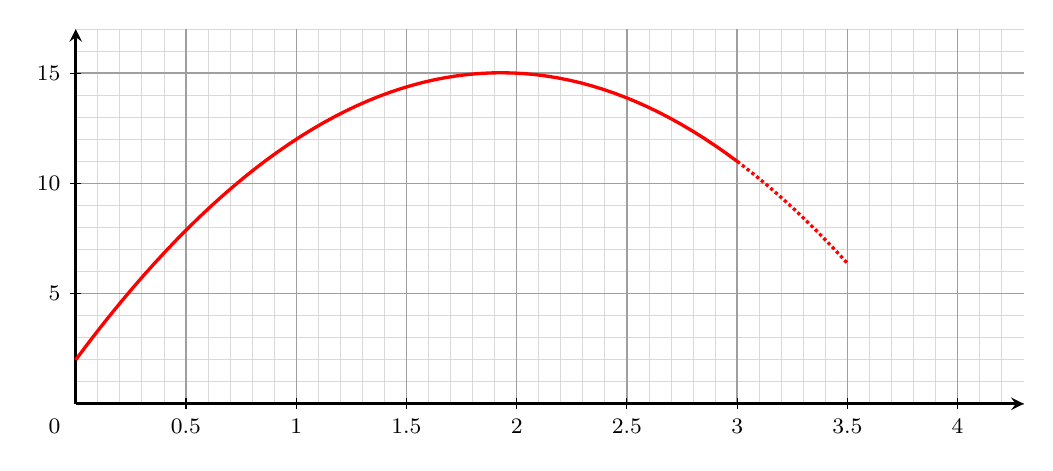
\begin{tikzpicture}[x=2.8cm,y=0.28cm,>=stealth]
			\draw[xstep=0.1,ystep=1,gray!30,line width=0.3pt] (0,0) grid (4.3,17);
			\draw[xstep=0.5,ystep=5,gray!75,line width=0.5pt] (0,0) grid (4.3,17);
			\draw[->,line width=1pt] (0,0) -- (4.3,0);
			\draw[->,line width=1pt] (0,0) -- (0,17);
			\foreach \x in {0.5,1,1.5,2,2.5,3,3.5,4} \draw (\x,2pt) -- (\x,-2pt) node[below] {\footnotesize \np{\x}};
			\foreach \y in {5,10,15} \draw (2pt,\y) -- (-2pt,\y) node[left] {\footnotesize \np{\y}};
			\draw (-2pt,-2pt) node[below left] {\footnotesize 0};
			\draw[line width=1.2pt,red] plot[domain=0:3,samples=60] (\x,{-3.5*\x*\x+13.5*\x+2});
			\draw[line width=1.2pt,red,densely dotted] plot[domain=3:3.5,samples=20] (\x,{-3.5*\x*\x+13.5*\x+2});
		\end{tikzpicture}

		\medskip

		\begin{tikzpicture}
			\tkzTabInit[lgt=3,espcl=2.5]{$t$/0.75,$f$/1.5}{$0$,$\frac{27}{14}$,$+\infty$}
			\tkzTabVar{-/{$2$},+/{},-/{}}
		\end{tikzpicture}
	\end{center}

	\begin{enumerate}
		\item Avec la précision permise par le graphique, déterminer l'intervalle de temps sur lequel la hauteur du projectile est supérieure ou égale à 12~m.
		\item À quel instant $t$ le projectile touchera-t-il le sol ? Justifier.
	\end{enumerate}
\end{enumerate}
